\documentclass[tikz]{standalone}
\begin{document}
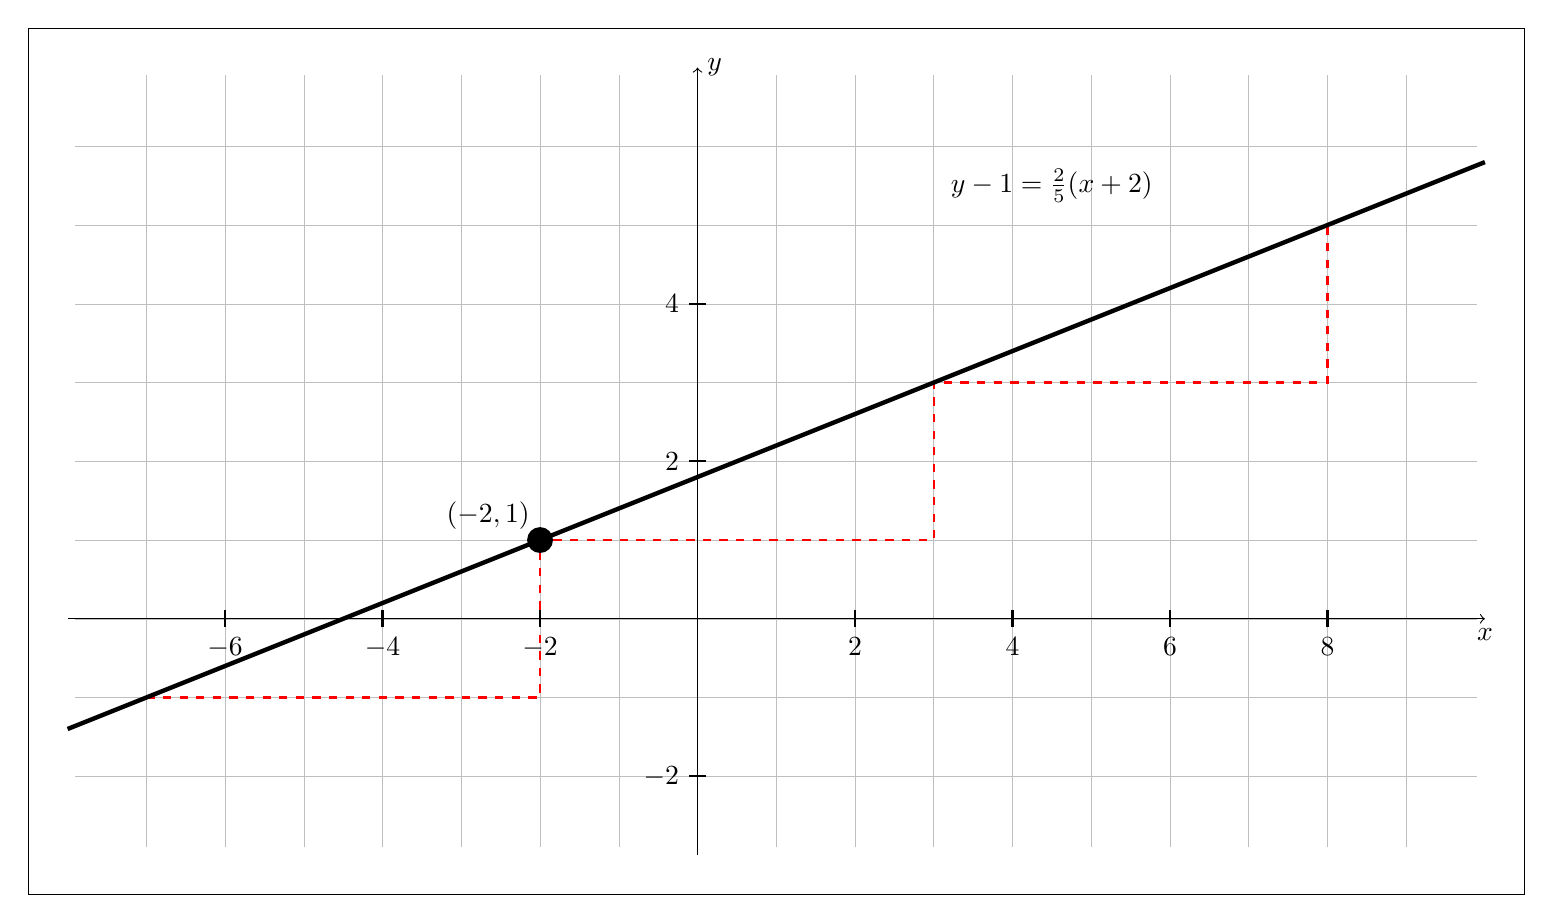
\begin{tikzpicture}[scale=1.0]
\draw[black,fill=white] (-8.5,-3.5) rectangle (10.5,7.5);
\draw[very thin,color=lightgray,step=1] (-7.9,-2.9) grid (9.9,6.9);
\draw[->] (-8,0) -- (10,0) node[below] {$x$};
\draw[->] (0,-3) -- (0,7) node[right] {$y$};
\node at (4.5, 5.5){$y - 1 = \frac{2}{5}(x+2)$};

% draw slope
\draw[dashed,red,thick] (-7,-1) -| ++(5,2) -| ++(5,2) -| ++(5,2);

% draw line and point
\draw[domain=-8:10,smooth,variable=\x,black,ultra thick] plot ({\x},{0.4*\x+9/5});
\draw [fill=black,thick] (-2,1) circle [radius=0.15] node [above left] {$(-2,1)$};

% tick marks
\foreach \x in {-6,-4,-2,2,4,6,8} 
	\draw [thick] (\x cm,3pt) -- (\x cm,-3pt) node[below] {$\x$};
\foreach \y in {-2,2,4} 
	\draw [thick] (3pt,\y cm) -- (-3pt,\y cm) node[left] {$\y$};
\end{tikzpicture}
\end{document}
